\chapter{Distorting Hinduism}

\begin{longtable}{|>{\raggedleft}p{1.5cm}|p{8.5cm}|}
\multicolumn{2}{c}{\textbf{Table: 1}}\\ 
\hline
\textbf{Page \#} & \textbf{McGraw Hill Text} \tabularnewline
\hline 
 261 & At first, the Vedas had to be memorized by Brahmin priests and spoken out loud. Much later, they were written down in Sanskrit. Over time, the Brahmin religion blended with the ideas of other people of India. This mix of beliefs eventually became known as Hinduism. \tabularnewline
\hline
\end{longtable}

\section*{Analysis and Critique} 

This is in violation of California Education Codes 51501 and 60044—adverse reflection—and evaluation criteria clauses pertaining to historical inaccuracy, not including variety of perspectives and debates, perpetrating Eurocentric and Ethnocentric history, not remaining neutral in matters of religion (continuing with the missionary and imperialistic writings on Hinduism), and thereby instilling prejudice in Hindu and non-Hindu children against origins of Hinduism and Hinduism per se.

These contentions are derogatory and factually incorrect. The preservers of the tradition, which now goes by the name of Hinduism, were Brahmins, and this tradition included people of all varnas and jatis. There was no separate religion of the Brahmins called Brahmanism, the use of which has been deleted from the current HSS framework. “Brahmin religion” is basically the euphemistic and politically correct use of “Brahmanism.” “Over time, the Brahmin religion blended with the ideas of other people of India. This mix of beliefs eventually became known as Hinduism” contains the following prejudices: 1. Hinduism is a social construction (it mixed with ideas of various populations and came into existence) and that it is not based on the revelations that the yogis and sages through their spiritual practices encountered. 2. Hinduism is a rag-tag collocation of many traditions stitched together by the machinations of the evil Brahmins, and its claims of any spiritual truth are spurious. Both these in-between-the-lines prejudices can be traced to the highly contentious writings of James Mill’s \textit{History of British India}, which was written with explicit imperialistic design containing myriad distortions on Indian History, culture, and Hinduism. 

\begin{longtable}{|>{\raggedleft}p{1.5cm}|p{8.5cm}|}
\multicolumn{2}{c}{\textbf{Table: 2}}\\ 
\hline
\textbf{Page \#} & \textbf{McGraw Hill Text} \tabularnewline
\hline
261 & Hinduism includes many beliefs and practices. Certain practices present in Hinduism today, such as worship in the home, worship in temples, yoga and meditation, developed over time. Acceptance of religious diversity also grew to be a central aspect of Hinduism. A core belief of Hinduism is that there is one universal spirit called Brahman (BRAH•muhn). Hindu teachings were spread orally at first. Over time they were written into texts like the Upanishads (oo•PAH•nih•shadz). The Upanishads describe the search for Brahman. These writings say that every living thing has a soul that is part of Brahman. The body is part of life on Earth. At death, the soul leaves the body and joins with Brahman. The Upanishads say that a soul that becomes one with Brahman is like a lump of salt thrown into water. The lump of salt is gone, but the water tastes salty. The salt has become part of the water. Most ancient Indians, however, could not easily understand the idea of Brahman. They believed in many different deities that were more like people. \tabularnewline
\hline
\end{longtable}

\section*{Analysis and Critique} 

These are in violation of California Education Codes 51501 and 60044—adverse reflection—and evaluation criteria clauses pertaining to historical inaccuracy, not including variety of perspectives and debates, perpetrating Eurocentric and Ethnocentric history, not remaining neutral in matters of religion (continuing with the missionary and imperialistic writings on Hinduism), and thereby instilling prejudice in Hindu and non-Hindu children regarding origins of Hinduism and Hinduism per se.

There are too many factually incorrect and derogatory statements in this single paragraph.
\begin{enumerate}
\itemsep=1pt
\item 
Considering the Vedas as separate from Hinduism is derogatory apart from being factually incorrect. The Upanishads are part of the Vedas—the fourth section of every Veda. When the oral tradition was alive, Vedas and Upanishads were transmitted orally from generation to generation. When the texts were written down, they were written down simultaneously. Further, the concept of pluralism and acceptance of religious diversity are core to Hinduism dating back to the Rig Veda which states that Truth is one—\textit{ekam sad viprah bahudha vadanti} meaning Truth is one, but the learned refer to it in different names—and did not develop over a period of time.\footnote{\textit{Rigveda} 1.164.46}
\item 
Brahman is not one universal spirit. It is one Being, which exists at transcendental, universal, and terrestrial levels. This basically means that there exists nothing but God in this universe—the God of course has many degrees and levels of manifestation. 
\item 
The Vedas and Upanishads were written simultaneously. The Upanishads come towards the end of the Vedas; therefore, they form part of what is called Vedanta, meaning texts that come towards the end of the Vedas. 
\item 
The Upanishads do not describe the search for Brahman. They describe how a seeker can realize or discover Brahman for himself or herself. 
\item 
Every soul is not part of Brahman—it is the Brahman itself. One of the chief claims of the tradition is that atman (which has been loosely described as soul) is Brahman. 
\item 
At death soul does not join Brahman. Soul already is Brahman. However, the soul has many layers of covering which does not allow it to know experientially that it is Brahman. These layers are rendered apart in human body through various spiritual practices like meditation and prayers. Once all the layers are removed, the soul knows that it Brahman, leading to a state of liberation which is called “moksha.” In such a state a soul gets to know that he or she is nothing but Brahman. Till such a state is reached, soul transmigrates from birth to birth, and death only is a temporary stage after which it takes a new body.
\item 
The quote about the soul being like salt is from the Brihadaranyaka Upanishad and is one of many different ways that the soul is described in the Upanishads. The present text implies this is the only description. There are however other texts and traditions in which the soul does not become one in God; all that it can have is a rapturous presence near God.
\item 
Multiple examples were provided to facilitate understanding of the underlying concepts by common people. Ritual and Deity worship was always parallel and co-existent with the philosophy of the Vedas and the Upanishads (multitudes of examples can be found in the Vedas and Upanishads themselves). 
\item 
It is a common Hindu understanding that various Deities are manifestations of one Brahman. It is incorrect and false to state that Deity worship arose due to people's inability to understand the concept of Brahman. Hinduism since antiquity has understood that people’s constitutions are different and that there cannot be one single way of approaching the Divine. The Divine in Hinduism has multiple aspects and there are multiple ways of approaching the Divine. 
\item 
It is derogatory to describe Deities to be “like people.” It gives a false impression that Hinduism is anthropomorphic religion.
\end{enumerate}

\begin{thebibliography}{99}

\bibitem{chap6-key1} Khandavalli, Shankara Bharadwaj. “Veda.” Hindupedia, the Hindu Encyclopedia. Accessed February 16, 2018. \url{http://www.hindupedia.com/en/Veda}.

\bibitem{chap6-key2} Ramachander, P.R. “Upanishad.” Hindupedia, the Hindu Encyclopedia. Accessed February 16, 2018. \url{http://www.hindupedia.com/en/Upanishad}.

\bibitem{chap6-key3} Singh, Kundan. \textit{The Evolution of Integral Yoga: Sri Ramakrishna, Swami Vivekananda, and Sri Aurobindo}. Saarbrucken, Germany: VDM Verlag, 2008.
\end{thebibliography}

\begin{longtable}{|>{\raggedleft}p{1.5cm}|p{8.5cm}|}
\multicolumn{2}{c}{\textbf{Table: 3}}\\ 
\hline
\textbf{Page \#} & \textbf{McGraw Hill Text} \tabularnewline
\hline
 262 & Hindus strive for moksha, the ultimate peace. \tabularnewline
\hline
\end{longtable}

\section*{Analysis and Critique} 

This violates the evaluation criterion of accuracy.

Moksha is incorrectly defined as “ultimate peace.” The correct definition is “freedom from the cycle of birth and death.”

\begin{longtable}{|>{\raggedleft}p{1.5cm}|p{8.5cm}|}
\multicolumn{2}{c}{\textbf{Table: 4}}\\ 
\hline
\textbf{Page \#} & \textbf{McGraw Hill Text} \tabularnewline
\hline
263 & Many Hindus today still believe that a man should go through four stages in his life: a student (preparing to live in the world), a married man (accepting worldly responsibilities), a forest dweller (retirement from the world), and, finally a wandering monk (completely renouncing the world). \tabularnewline
\hline
\end{longtable}


\section*{Analysis and Critique} 

This is in violation of California Education Codes 51501 and 60044—adverse reflection—and evaluation criteria clauses pertaining to historical inaccuracy, not including variety of perspectives and debates, perpetrating Eurocentric and Ethnocentric history, not remaining neutral in matters of religion (continuing with the missionary and imperialistic writings on Hinduism), and thereby instilling prejudice in Hindu and non-Hindu children against origins of Hinduism and Hinduism per se. 

Inaccurate as it incorrectly defines the four ashramas or stages of life. The third stage of life, vanaprastha, is not defined as a forest dweller. It is defined as one in which one readies himself or herself to depart to the forest.

As per the Hindu scriptures, during this stage of life, one goes into seclusion, and does penance. One becomes inward looking and gradually prepares for the final stage of sanyasa in which the objective is to gain moksha or liberation. He or she still contributes to the society with his experience, through advising and teaching—yes there were women hermits as well in Ancient India (see Kautilya’s \textit{Arthashastra} for details). Having fulfilled one’s desires in the previous ashrama, one is expected to win over senses and sensuous pleasures. Thus, one’s work is also more dispassionate and detached, as one does not seek any specific result from the work. It will be for the benefit of society alone. Though one is supposed to be celibate, one is not required to renounce or live alone. One can be with one’s spouse or live with any other person. But unless there is a specific need, one does not visit people—usually people needing a vanaprasthi's advice go to him or her.\footnote{Shankara Bharadwaj Khandavalli,“Varna Ashrama Dharma,” Hindupedia, the Hindu Encyclopedia, accessed February 16, 2018. \url{http://www.hindupedia.com/en/Varna_Ashrama_Dharma}.}

One of the recurring themes of colonial and missionary writing was to represent Hinduism as an otherworldly religion. As a part of that agenda, the Vanaprastha stage of life was inaccurately represented as one of forest dweller. The missionaries used this representation to convert and the colonialist to control—after all, if a population is told repeatedly that its traditions have been otherworldly, then it is easier to control. The McGraw Hill text regurgitates the orientalist and missionary agenda, misrepresenting and distorting Hinduism, thus instilling prejudice among its readers. As a result it adversely reflects on it and indoctrinates readers against it. 
\vskip -5pt

\begin{longtable}{|>{\raggedleft}p{1.5cm}|p{8.5cm}|}
\multicolumn{2}{c}{\textbf{Table: 5}}\\ 
\hline
\textbf{Page \#} & \textbf{McGraw Hill Text} \tabularnewline
\hline
248, 255, 261 & deities \tabularnewline
\hline
275 & The ancient Hindus believed that music was a gift from the gods. \tabularnewline
\hline
\end{longtable}
\vskip -15pt

\section*{Analysis and Critique} 
\vskip -4pt

These are in violation of California Education Codes 51501 and 60044 - adverse reflection.

The CAPEEM Lawsuit ruled against the State of CA in 2006 with a statement that lower-case use of “d” for Deities and “g” for Gods is discriminatory and indicates that Hindu Deities and Gods are inferior to the Abrahamic God. Further, Hindus believe everything beautiful and sublime is a gift of God, not just music.

The use of lower case for Deities and Gods basically conflates Hinduism with polytheism, and in the binary of monotheism/polytheism, privileges monotheism over polytheism.
\vskip -10pt

\begin{longtable}{|>{\raggedleft}p{1.5cm}|p{8.5cm}|}
\multicolumn{2}{c}{\textbf{Table: 6}}\\ 
\hline
\textbf{Page \#} & \textbf{McGraw Hill Text} \tabularnewline
\hline
 260 & \centering\vbox{\kern4pt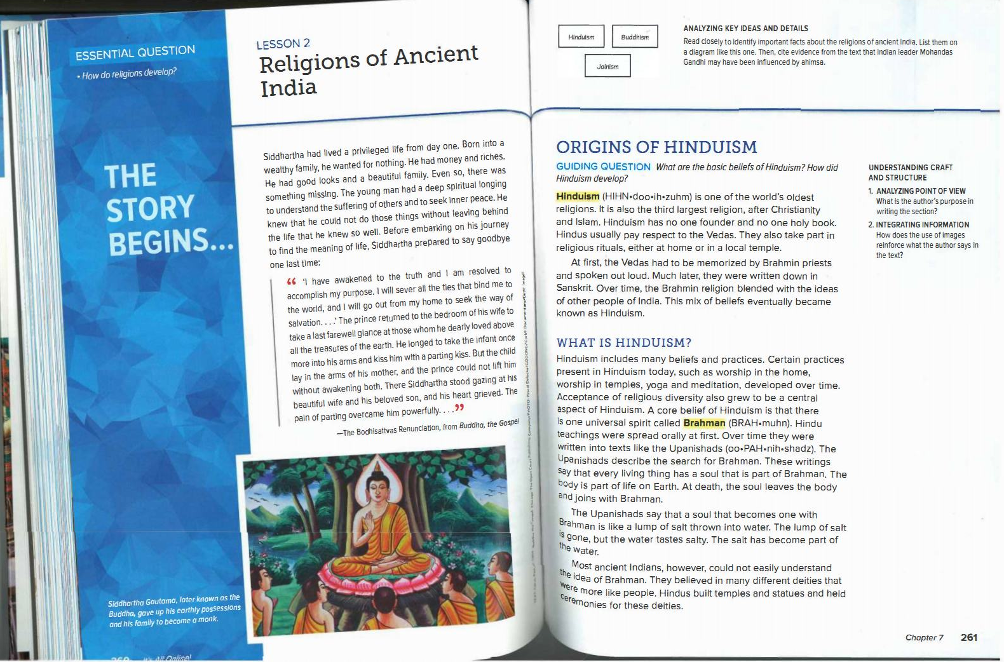
\includegraphics[scale=0.7]{figures/chap6-fig1.png}\kern4pt} \tabularnewline
\hline
\end{longtable}

\section*{Analysis and Critique} 

This is in violation of evaluation criterion pertaining to a proper sequencing of historical events–history is a story well told “with continuity and narrative coherence (a beginning, a middle, and an end)”.

The section on religions of Ancient India starting with Hinduism begins with a story about the Buddha which messes up the story. This story of Hinduism does not begin with Buddhism and yet that is what is presented. The HSS framework requires history to be presented as a story well told, with continuity and narrative coherence (a beginning, a middle, and an end).

